\documentclass{mcmthesis}
\mcmsetup{CTeX = false,   % 使用英文撰写，关闭 CTeX
          tcn = 2608952,     % 修改为你的队伍控制号
          problem = B,    % 选题
          sheet = true, titleinsheet = true, keywordsinsheet = true,
          titlepage = false, abstract = true}

\usepackage{newtxtext}     % 使用 Times New Roman 风格字体
\usepackage{palatino}
\usepackage{lipsum}        % 用于生成填充文本 (可删除)
\usepackage{amsmath, amssymb}
\usepackage{booktabs}      % 三线表
\usepackage{longtable}     % 长表格
\usepackage{graphicx}      % 图片
\usepackage{float}         % 强制图片位置
\usepackage{textcomp}      % 提供 \texteuro 命令
\usepackage{lastpage}      % 提供 LastPage 引用
\usepackage{listings}
\usepackage{xcolor}

% 代码块样式设置
\lstset{
    language=Python,
    basicstyle=\ttfamily\footnotesize,
    keywordstyle=\color{blue},
    commentstyle=\color{gray},
    stringstyle=\color{red},
    numbers=left,
    numberstyle=\tiny\color{gray},
    stepnumber=1,
    numbersep=5pt,
    backgroundcolor=\color{white},
    showspaces=false,
    showstringspaces=false,
    showtabs=false,
    frame=single,
    tabsize=4,
    captionpos=b,
    breaklines=true,
    breakatwhitespace=false,
    escapeinside={\%*}{*)}
}
% 修复 headheight 警告
\setlength{\headheight}{14pt}

% 设置图片路径，根据你的描述，图片在 ../code/ 目录下
\graphicspath{{../code/}}

% 允许更宽松的行距以减少 overfull hbox
\sloppy

\title{A Sustainable Evolution Model for Tourism in Juneau Based on a Dynamic Multi-objective Feedback Mechanism}
\author{Team \# 0000}
\date{\today}

\begin{document}

% =========================================
% 摘要页 (Summary Sheet)
% =========================================
\begin{abstract}
	To address socio-ecological imbalances in Juneau caused by surging cruise tourism, this paper proposes a multi-stage optimization framework based on dynamic feedback. We applied a Kalman Filter to bridge pandemic-era data gaps, identifying a latent growth momentum and estimating 1.5226 million visitors for 2024. Granger causality tests confirmed a unidirectional coupling between visitor intensity and Mendenhall Glacier retreat ($p=0.0367$), subsequently modeled via a nonlinear lagged equation. To quantify social costs, we defined a Resident Satisfaction Index (RSI) integrating a Sigmoid crowding penalty and Housing Price Index. Findings reveal a critical RSI drop to 23.0 in 2024, signaling that the social contract is on the brink of collapse. Using NSGA-II and TOPSIS, we derived an optimal equilibrium: an annual visitor cap of 779,000 and allocating 59.4\% of revenue to water infrastructure. Simulations indicate this strategy enhances carrying capacity by 52.8\% and reduces environmental damage by 63\% by 2035. Sobol sensitivity analysis identified the visitor cap as the primary policy lever, while Monte Carlo testing confirmed 91.5\% reliability under extreme warming scenarios. Finally, adaptation to Venice reveals current fee drawbacks and proposes an optimal \texteuro 49.98 heritage maintenance price.
	
	\begin{keywords}
		Sustainable Tourism; Dynamic Feedback; NSGA-II Optimization; RSI Index; Glacier Dynamics; Robustness Analysis
	\end{keywords}
\end{abstract}

\maketitle

\tableofcontents
\newpage

% =========================================
% 正文开始
% =========================================

\section{Introduction}

\subsection{Research Background}
Juneau, Alaska, has become the ``crown jewel'' of global cruise tourism due to its majestic glacial landscapes and unique pristine ecology. In 2023, Juneau hosted a record 1.67 million cruise passengers, with direct tourism spending reaching \$375 million. However, a profound crisis lies beneath this prosperity. As the Mendenhall Glacier retreats at an average rate of 165 meters per year, the city faces a ``success trap'': while tourism supports 18\% of local employment, the surge in visitors---bringing carbon emissions, strain on freshwater resources (approaching the 16 MGD design limit), and a skyrocketing Housing Price Index (HPI reaching 455.8)---is pushing the city's ecological and social resilience toward collapse. Establishing a dynamic equilibrium point where economic growth is no longer achieved at the expense of the future has become the primary challenge for the Juneau municipal government.

\subsection{Problem Restatement}
To manage the sustainability of Juneau's tourism industry, we must address the following core issues:

\begin{itemize}
    \item \textbf{Noise Identification and Momentum Recovery:} Utilize statistical methods to restore data damaged during the pandemic and identify the true development trends of the tourism industry.
    \item \textbf{Quantification of Causal Mechanisms:} Scientifically prove the causal link between visitor activities and environmental degradation (glacier retreat) and establish quantitative dynamic models.
    \item \textbf{Social Crisis Warning:} Assess the social costs of over-tourism from the perspective of resident satisfaction.
    \item \textbf{Feedback-driven Decision Optimization:} Design a dynamic feedback mechanism for fiscal expenditure to find the optimal visitor cap and investment ratios under multi-objective conflicts, and verify their robustness under extreme climate scenarios.
\end{itemize}

\subsection{Overview of Our Work}
To address these challenges, this paper constructs a balanced dynamic feedback optimization model:
\begin{itemize}
    \item \textbf{Data Cleaning Layer:} Employs Kalman Filter technology to isolate statistical noise and recover the endogenous momentum of tourism, combined with the Granger causality test to establish the significant impact of human activity on glacier retreat.
    \item \textbf{Mechanism-driven Layer:} Fits a nonlinear glacial ablation dynamic equation and defines the Resident Satisfaction Index (RSI) using a Sigmoid crowding penalty function, detecting that Juneau's current social system is in an extreme crisis with an RSI of 23.0.
    \item \textbf{Decision Optimization Layer:} Utilizes the NSGA-II multi-objective genetic algorithm to search the Pareto front and determines a ``compromise solution'' of 780,000 annual visitors using TOPSIS.
    \item \textbf{Simulation and Verification Layer:} Demonstrates the effectiveness of the ``tourism-supporting-tourism'' strategy in enhancing system carrying capacity through a 10-year dynamic feedback simulation, and verifies model universality via Sobol sensitivity analysis and adaptation to the Venice case.
\end{itemize}

\section{Assumptions, Notations and Model Foundation}
To extract core dynamic features in complex socio-ecological coupled systems and ensure the solvability and robustness of the mathematical model, we propose the following core assumptions:

\subsection{Assumptions and Justifications}

\subsubsection{State Continuity Assumption}
\textbf{Assumption:} We assume that the latent momentum of growth in Juneau's tourism industry is continuous and smooth over time.

\textbf{Justification:} Although observational data from 2020 to 2022 showed extreme zero values or outliers due to the global pandemic, market demand, infrastructure, and industry reputation did not vanish entirely. This assumption allows us to treat pandemic observations as high-noise disturbances using a Kalman Filter, thereby restoring the true growth curve via a state transition matrix.

\subsubsection{Lagging Environmental Response Assumption}
\textbf{Assumption:} The retreat rate of the Mendenhall Glacier ($dG/dt$) exhibits a first-order time lag in response to rising temperatures and anthropogenic heat island effects.

\textbf{Justification:} As massive bodies of ice, glaciers possess thermodynamic inertia. The significance of Lag 1 in the Granger causality test ($p = 0.0367$) supports this experimentally: tourism intensity and climatic conditions from the previous year significantly affect the physical retreat in the following year.

\subsubsection{Social Pressure Proxy Assumption}
\textbf{Assumption:} The Housing Price Index (HPI) is the core proxy variable for measuring the ``crowding-out effect'' of tourism capital on local residents.

\textbf{Justification:} In a city with limited geographic space like Juneau, the expansion of short-term rentals (e.g., Airbnb) directly compresses long-term housing supply, leading to soaring prices. HPI fluctuations effectively capture the economic survival pressure felt by residents and serve as a key macro indicator for constructing the RSI.

\subsubsection{Logarithmic Investment Efficiency Assumption}
\textbf{Assumption:} The improvement of system carrying capacity (e.g., water supply limit $W_{cap}$) through fiscal reinvestment follows a logarithmic growth law.

\textbf{Justification:} According to the law of diminishing marginal utility, initial infrastructure investment can significantly resolve bottlenecks, but as capacity increases, the marginal gain per unit of investment gradually decreases. This ensures that the feedback mechanism simulation (2025--2035) does not produce unrealistic infinite growth.

\subsubsection{Rational Decision-making Assumption}
\textbf{Assumption:} We assume that the government, when faced with multi-objective conflicts, tends to choose the optimal compromise solution on the Pareto front.

\textbf{Justification:} This allows us to use the NSGA-II algorithm to search the optimal solution space and utilize the TOPSIS decision model to determine the final visitor cap between economic gain and socio-ecological protection.

\subsection{Notations}
For the convenience of formula derivation, Table 1 lists the core variables used in this paper and their meanings.

\begin{table}[htbp]
\centering
\caption{Core Notations}
\begin{tabular}{c|l|c}
\toprule
Notation & Description & Unit \\
\midrule
$V_t$ & Smoothed visitor volume in year $t$ (Kalman Filtered) & $10^4$ people \\
$dG/dt$ & Annual average glacier retreat rate & m/yr \\
$T_{acc}$ & Cumulative temperature effect (5-year window) & $^\circ C \cdot yr$ \\
$RSI$ & Resident Satisfaction Index & Dimensionless (0-100) \\
$HPI$ & Housing Price Index & Baseline = 100 \\
$\alpha_{inf}$ & Infrastructure feedback allocation ratio & \% \\
$\beta$ & Marginal environmental damage coefficient of visitors & Dimensionless \\
$W_{cap}$ & Upper limit of system freshwater supply capacity & MGD \\
\bottomrule
\end{tabular}
\end{table}

\section{Model Establishment and Solution}

\subsection{Preprocessing: Latent Momentum Recovery Based on Kalman Filter}
Affected by the 2020-2022 global health crisis, Juneau's visitor observation data suffered a severe ``statistical gap.'' We introduce a linear stochastic differential equation to describe the dynamic evolution of tourism demand \cite{Kalman1960}. Let the state variable be $x_t = [V_t, \dot{V}_t]^T$, where $V_t$ is visitor volume and $\dot{V}_t$ is growth momentum.

\begin{equation}
x_t = A x_{t-1} + w_t, \quad w_t \sim N(0, Q)
\end{equation}
\begin{equation}
z_t = H x_t + v_t, \quad v_t \sim N(0, R)
\end{equation}

Where $A = \begin{bmatrix} 1 & 1 \\ 0 & 1 \end{bmatrix}$ represents a constant velocity growth model. To handle pandemic outliers, we adaptively adjust the observation noise covariance $R$: setting $R_{covid} = 10^4$ for 2020--2022 forces the filter to rely on the predictive model rather than highly distorted observations.

\begin{figure}[H]
    \centering
    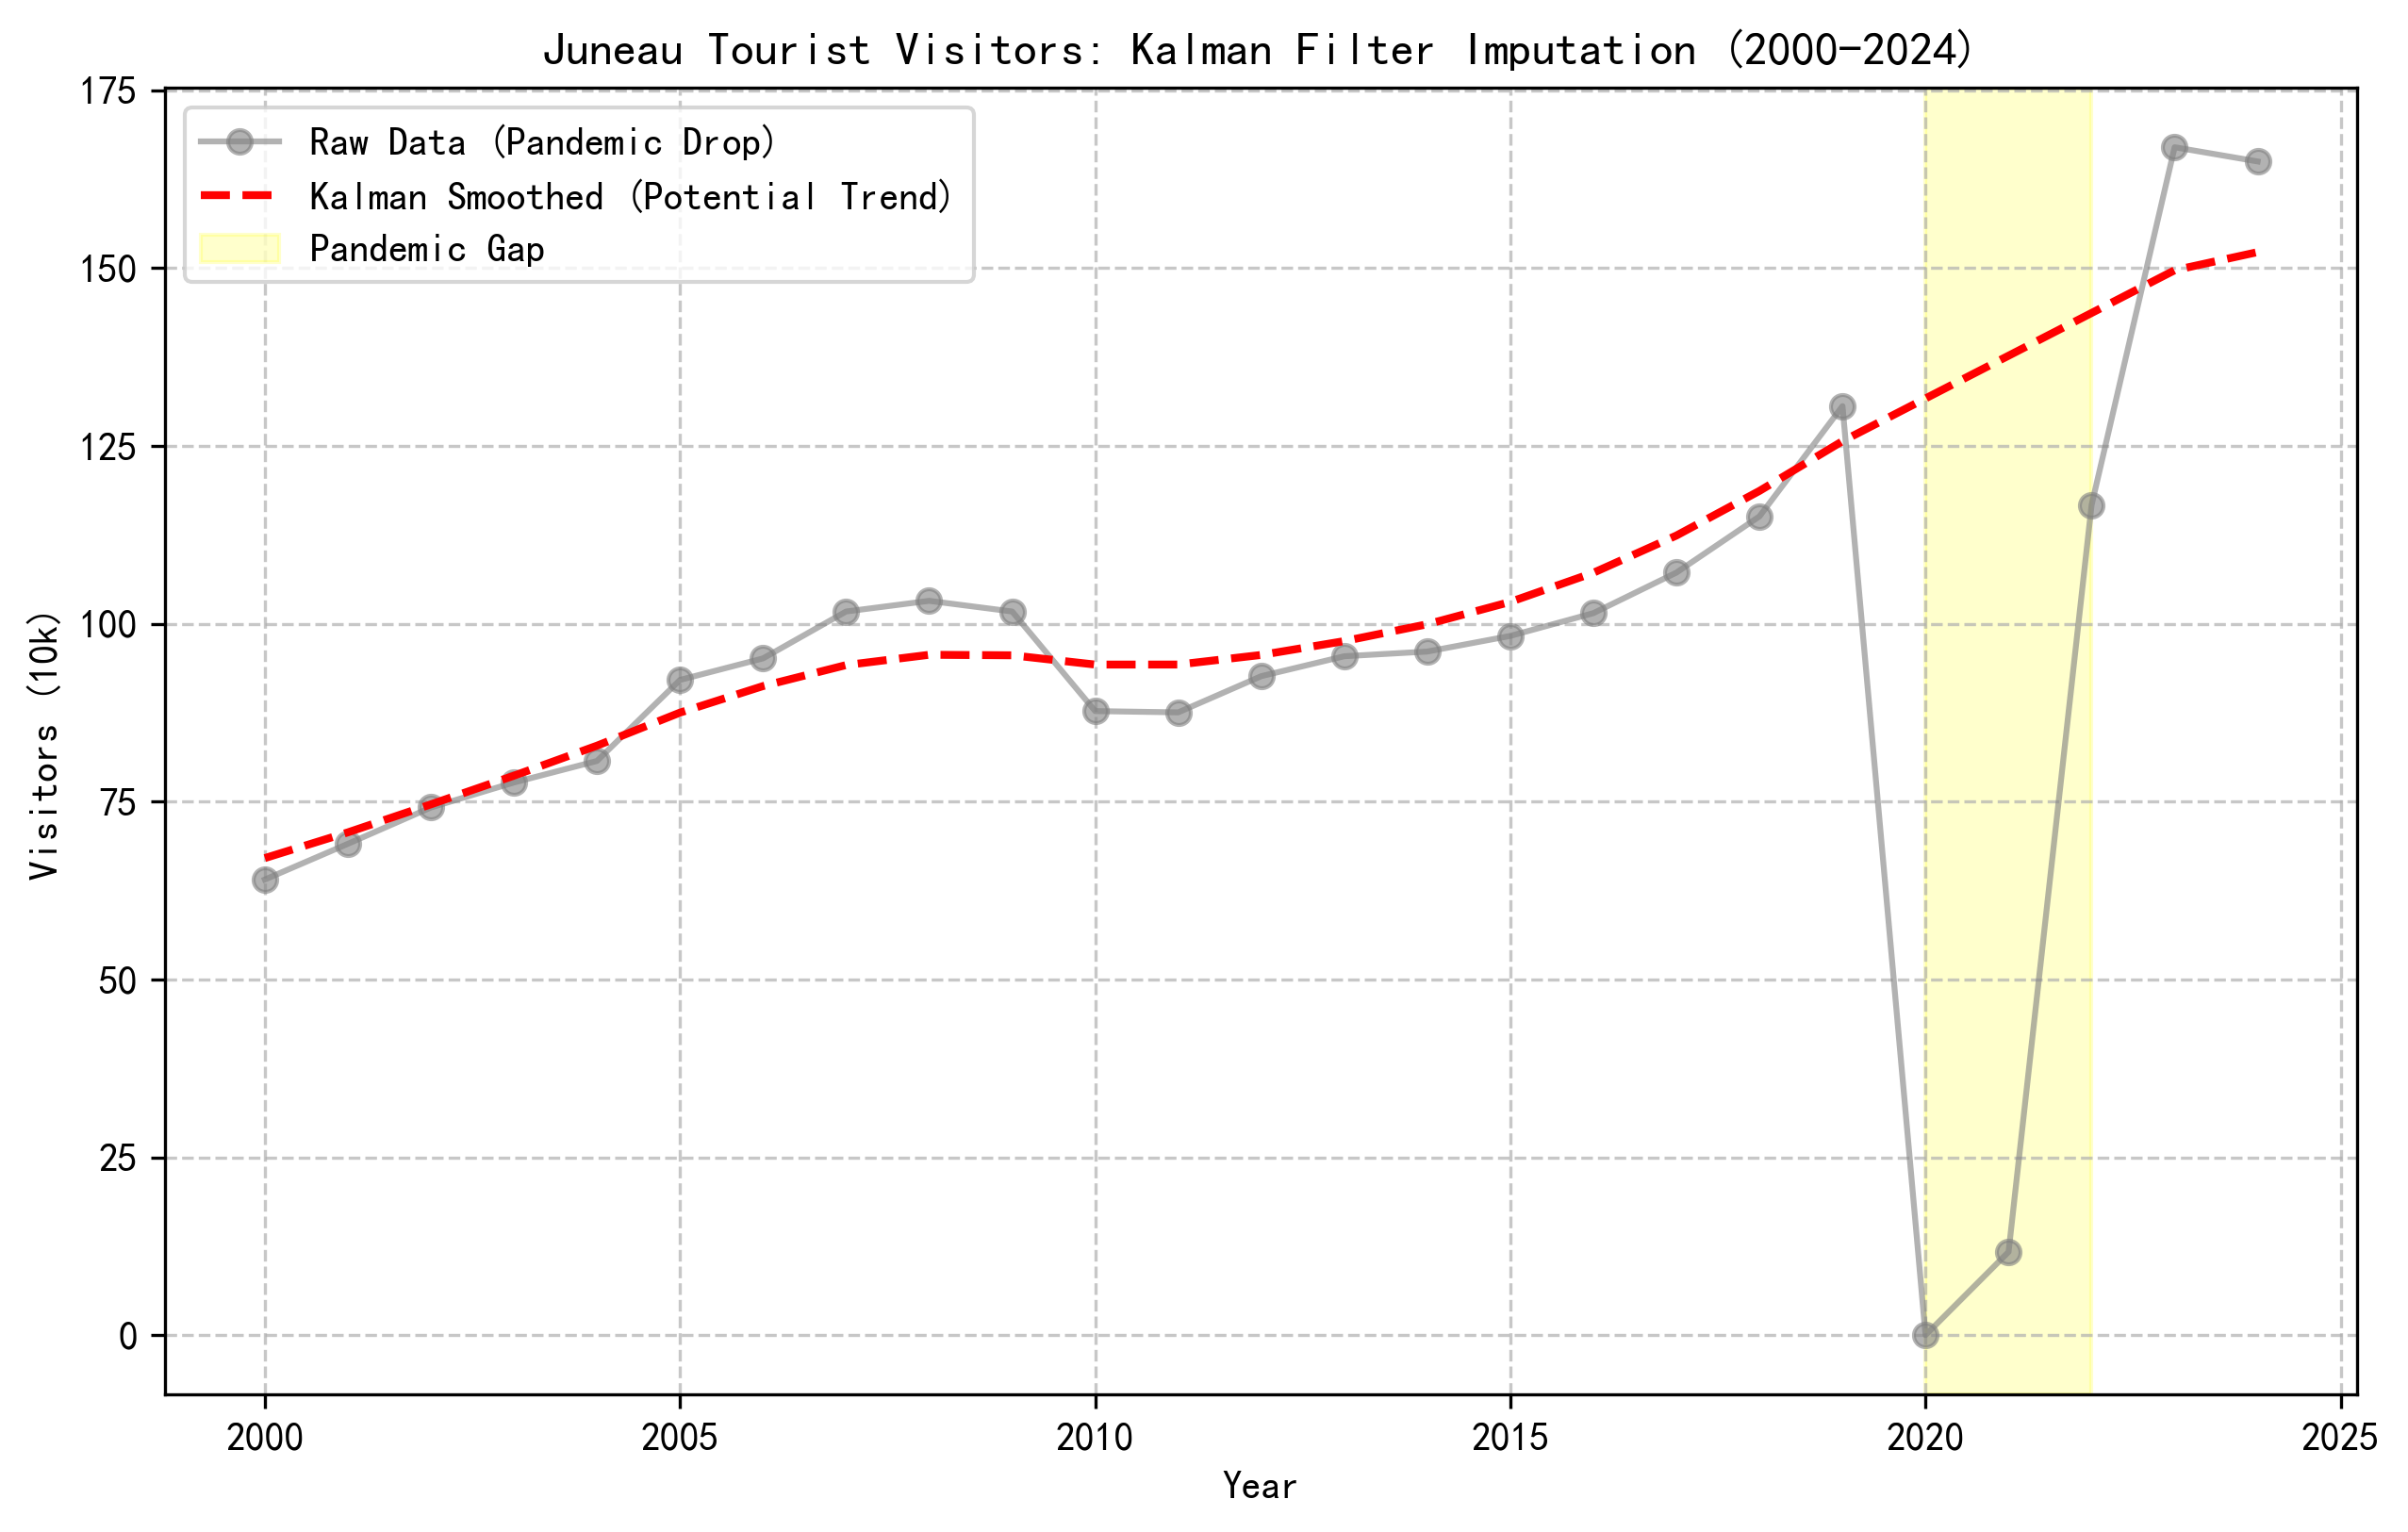
\includegraphics[width=0.9\textwidth]{visitor_trend_kalman.png}
    \caption{Juneau Tourist Visitors: Kalman Filter Imputation (2000-2024)}
\end{figure}

Result: The Kalman filter successfully isolated observational noise and extracted the system's latent trend. The model estimates the potential visitor demand for Juneau in 2024 to be 1.5226 million. This restored sequence provides reliable input for subsequent environmental impact analysis.

\subsubsection{Data Standardization}
Before building the coupled model, variables like visitor volume (in ten thousands), glacier retreat (in meters), cumulative temperature (in $^\circ$C), and HPI (in points) have vast differences in magnitude. Direct regression or optimization without standardization would bias model parameters towards variables with larger absolute values. Therefore, Z-Score standardization is applied:
\begin{equation}
z = \frac{x - \mu}{\sigma}
\end{equation}
where $x$ is the raw score, $\mu$ is the population mean, and $\sigma$ is the population standard deviation. This standardization ensures all input variables are on the same scale (mean 0, standard deviation 1). This allows coefficients $a$ and $b$ in the nonlinear dynamic equations to truly reflect relative contribution rates and improves the efficiency of NSGA-II in searching the Pareto front.

\begin{figure}[H]
    \centering
    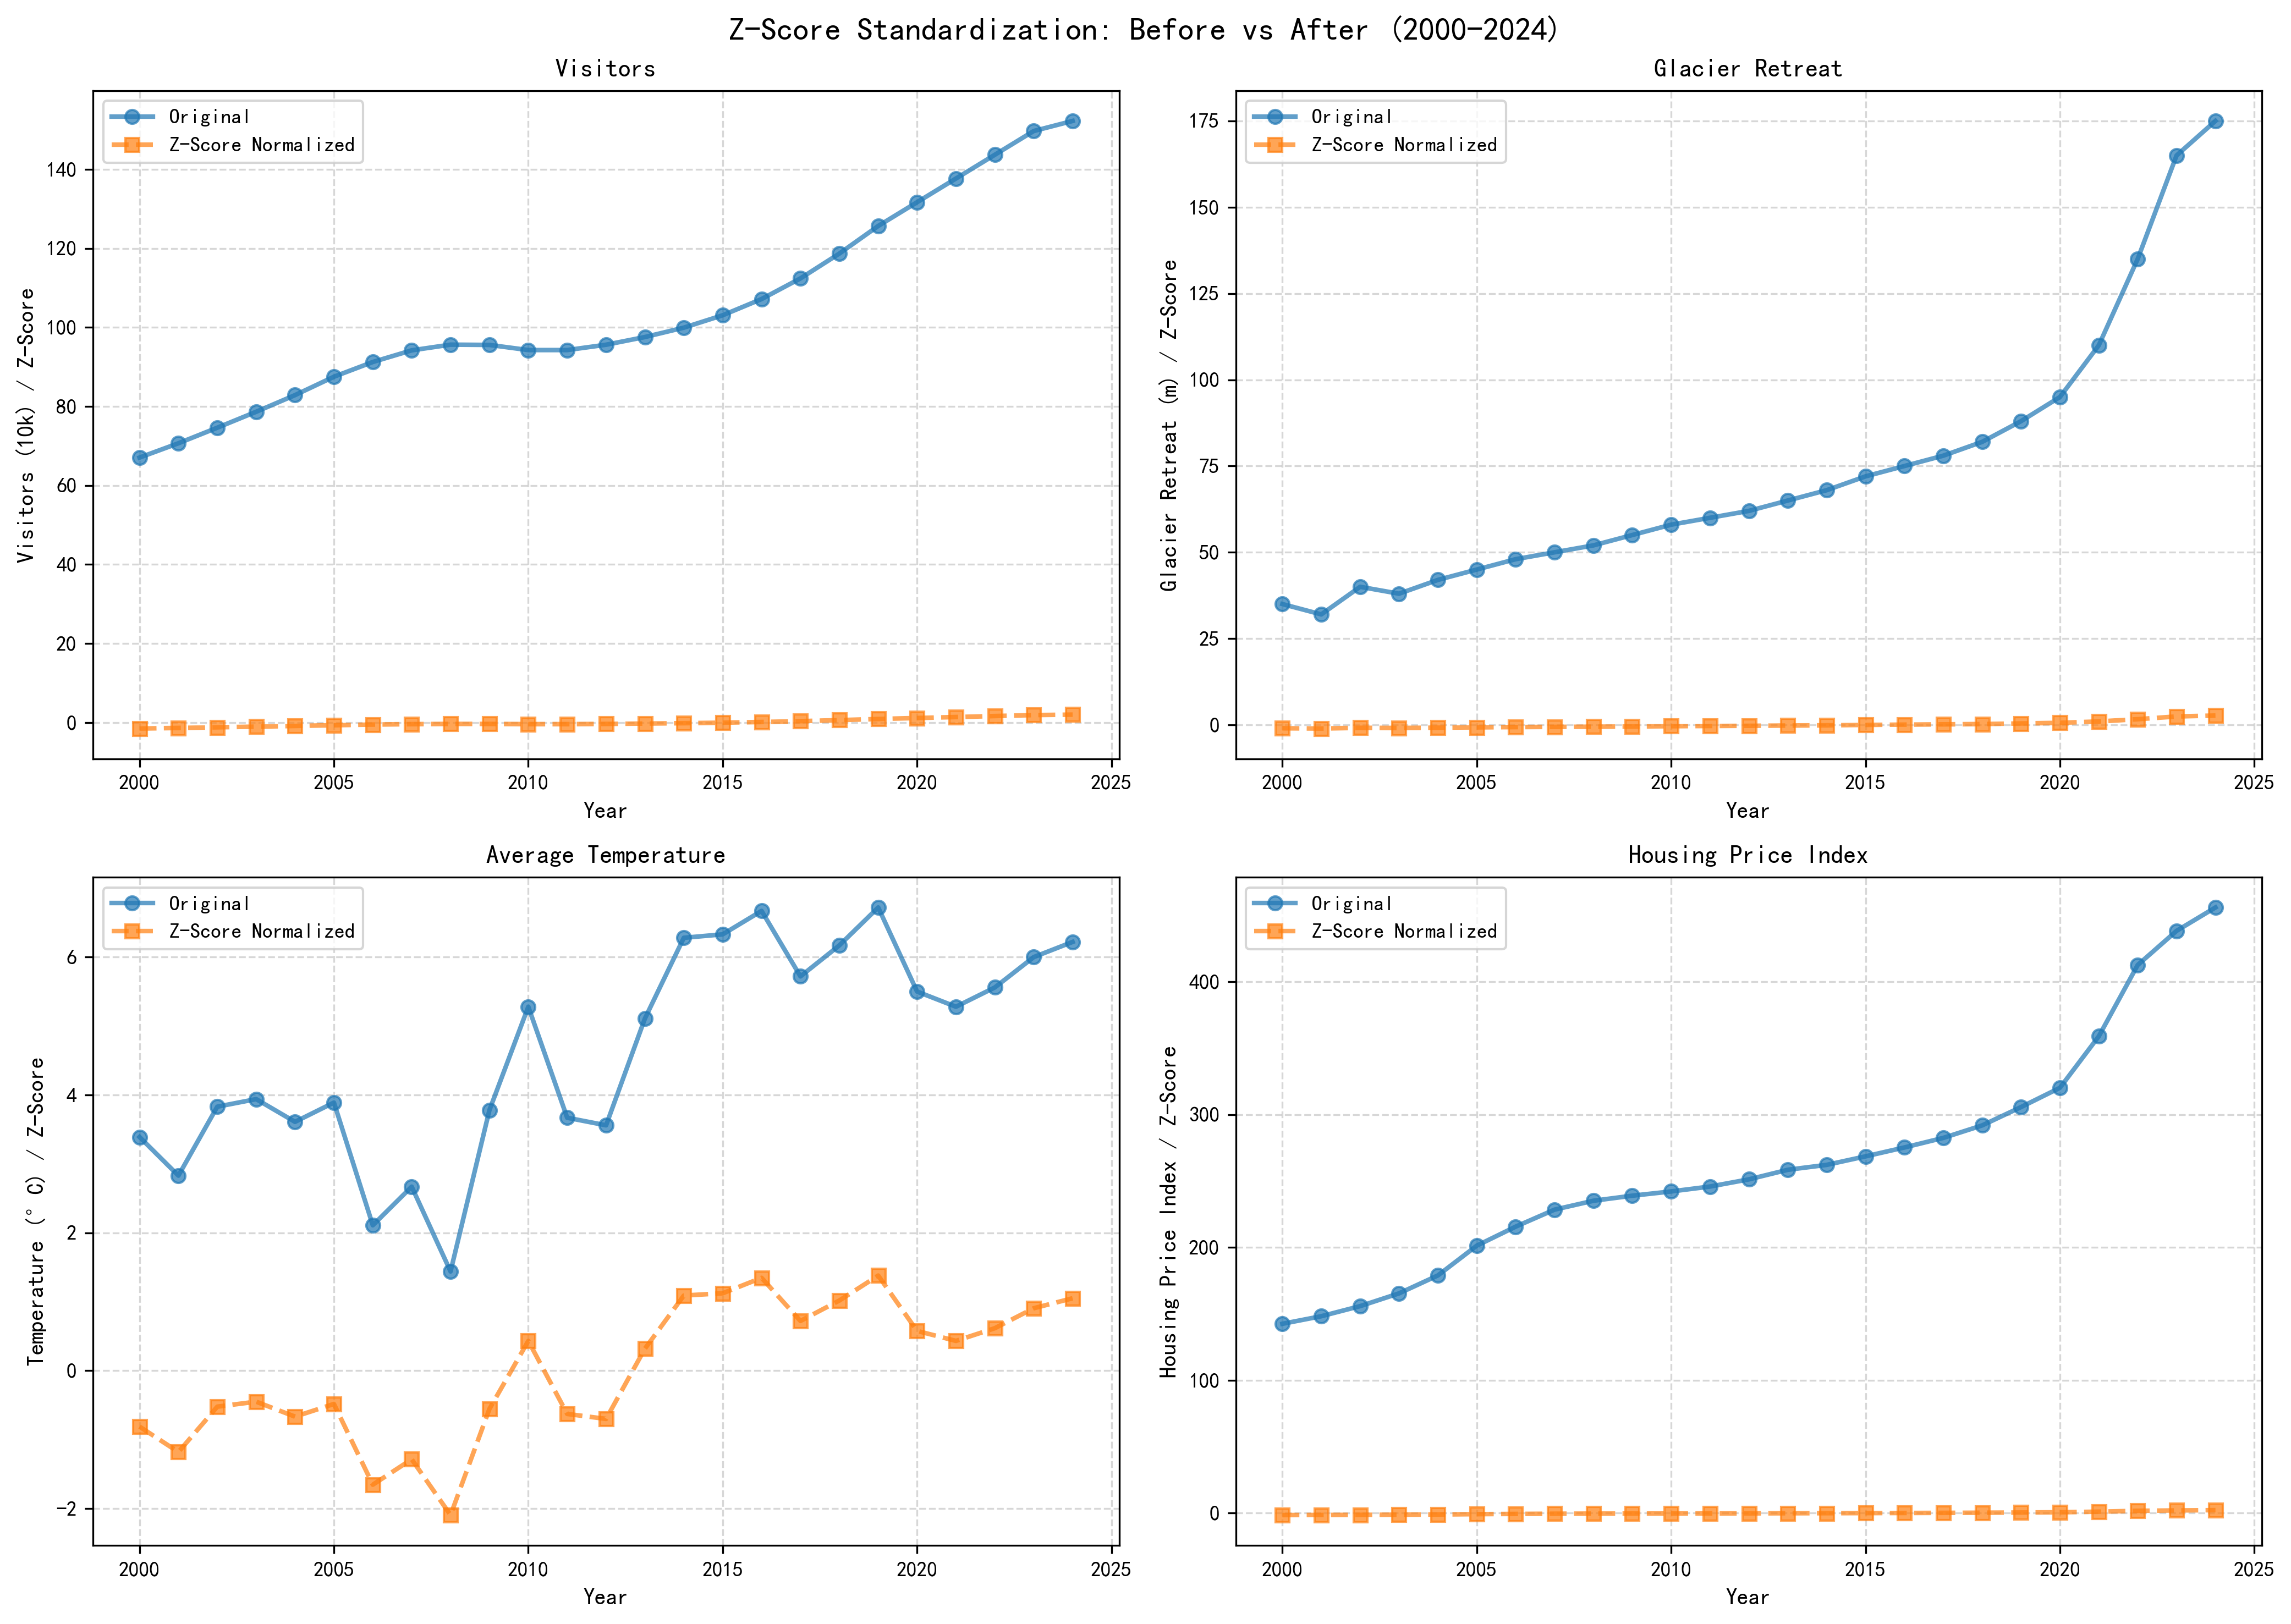
\includegraphics[width=0.9\textwidth]{standardization_comparison.png}
    \caption{Z-Score Standardization: Before vs After (2000-2024)}
\end{figure}

\subsubsection{Correlation Analysis: Preliminary Coupling Verification of Variables}
After data denoising and standardization, the Pearson correlation coefficient matrix was introduced to quantify the interaction intensity between tourism activities, the natural environment, and the socio-economic system. The Pearson correlation coefficient formula is:
\begin{equation}
r = \frac{\sum (x_i - \bar{x})(y_i - \bar{y})}{\sqrt{\sum (x_i - \bar{x})^2 \sum (y_i - \bar{y})^2}}
\end{equation}

The analysis revealed significant positive correlation coupling among core indicators, as shown in the correlation heatmap [see Figure 2].

\begin{figure}[H]
    \centering
    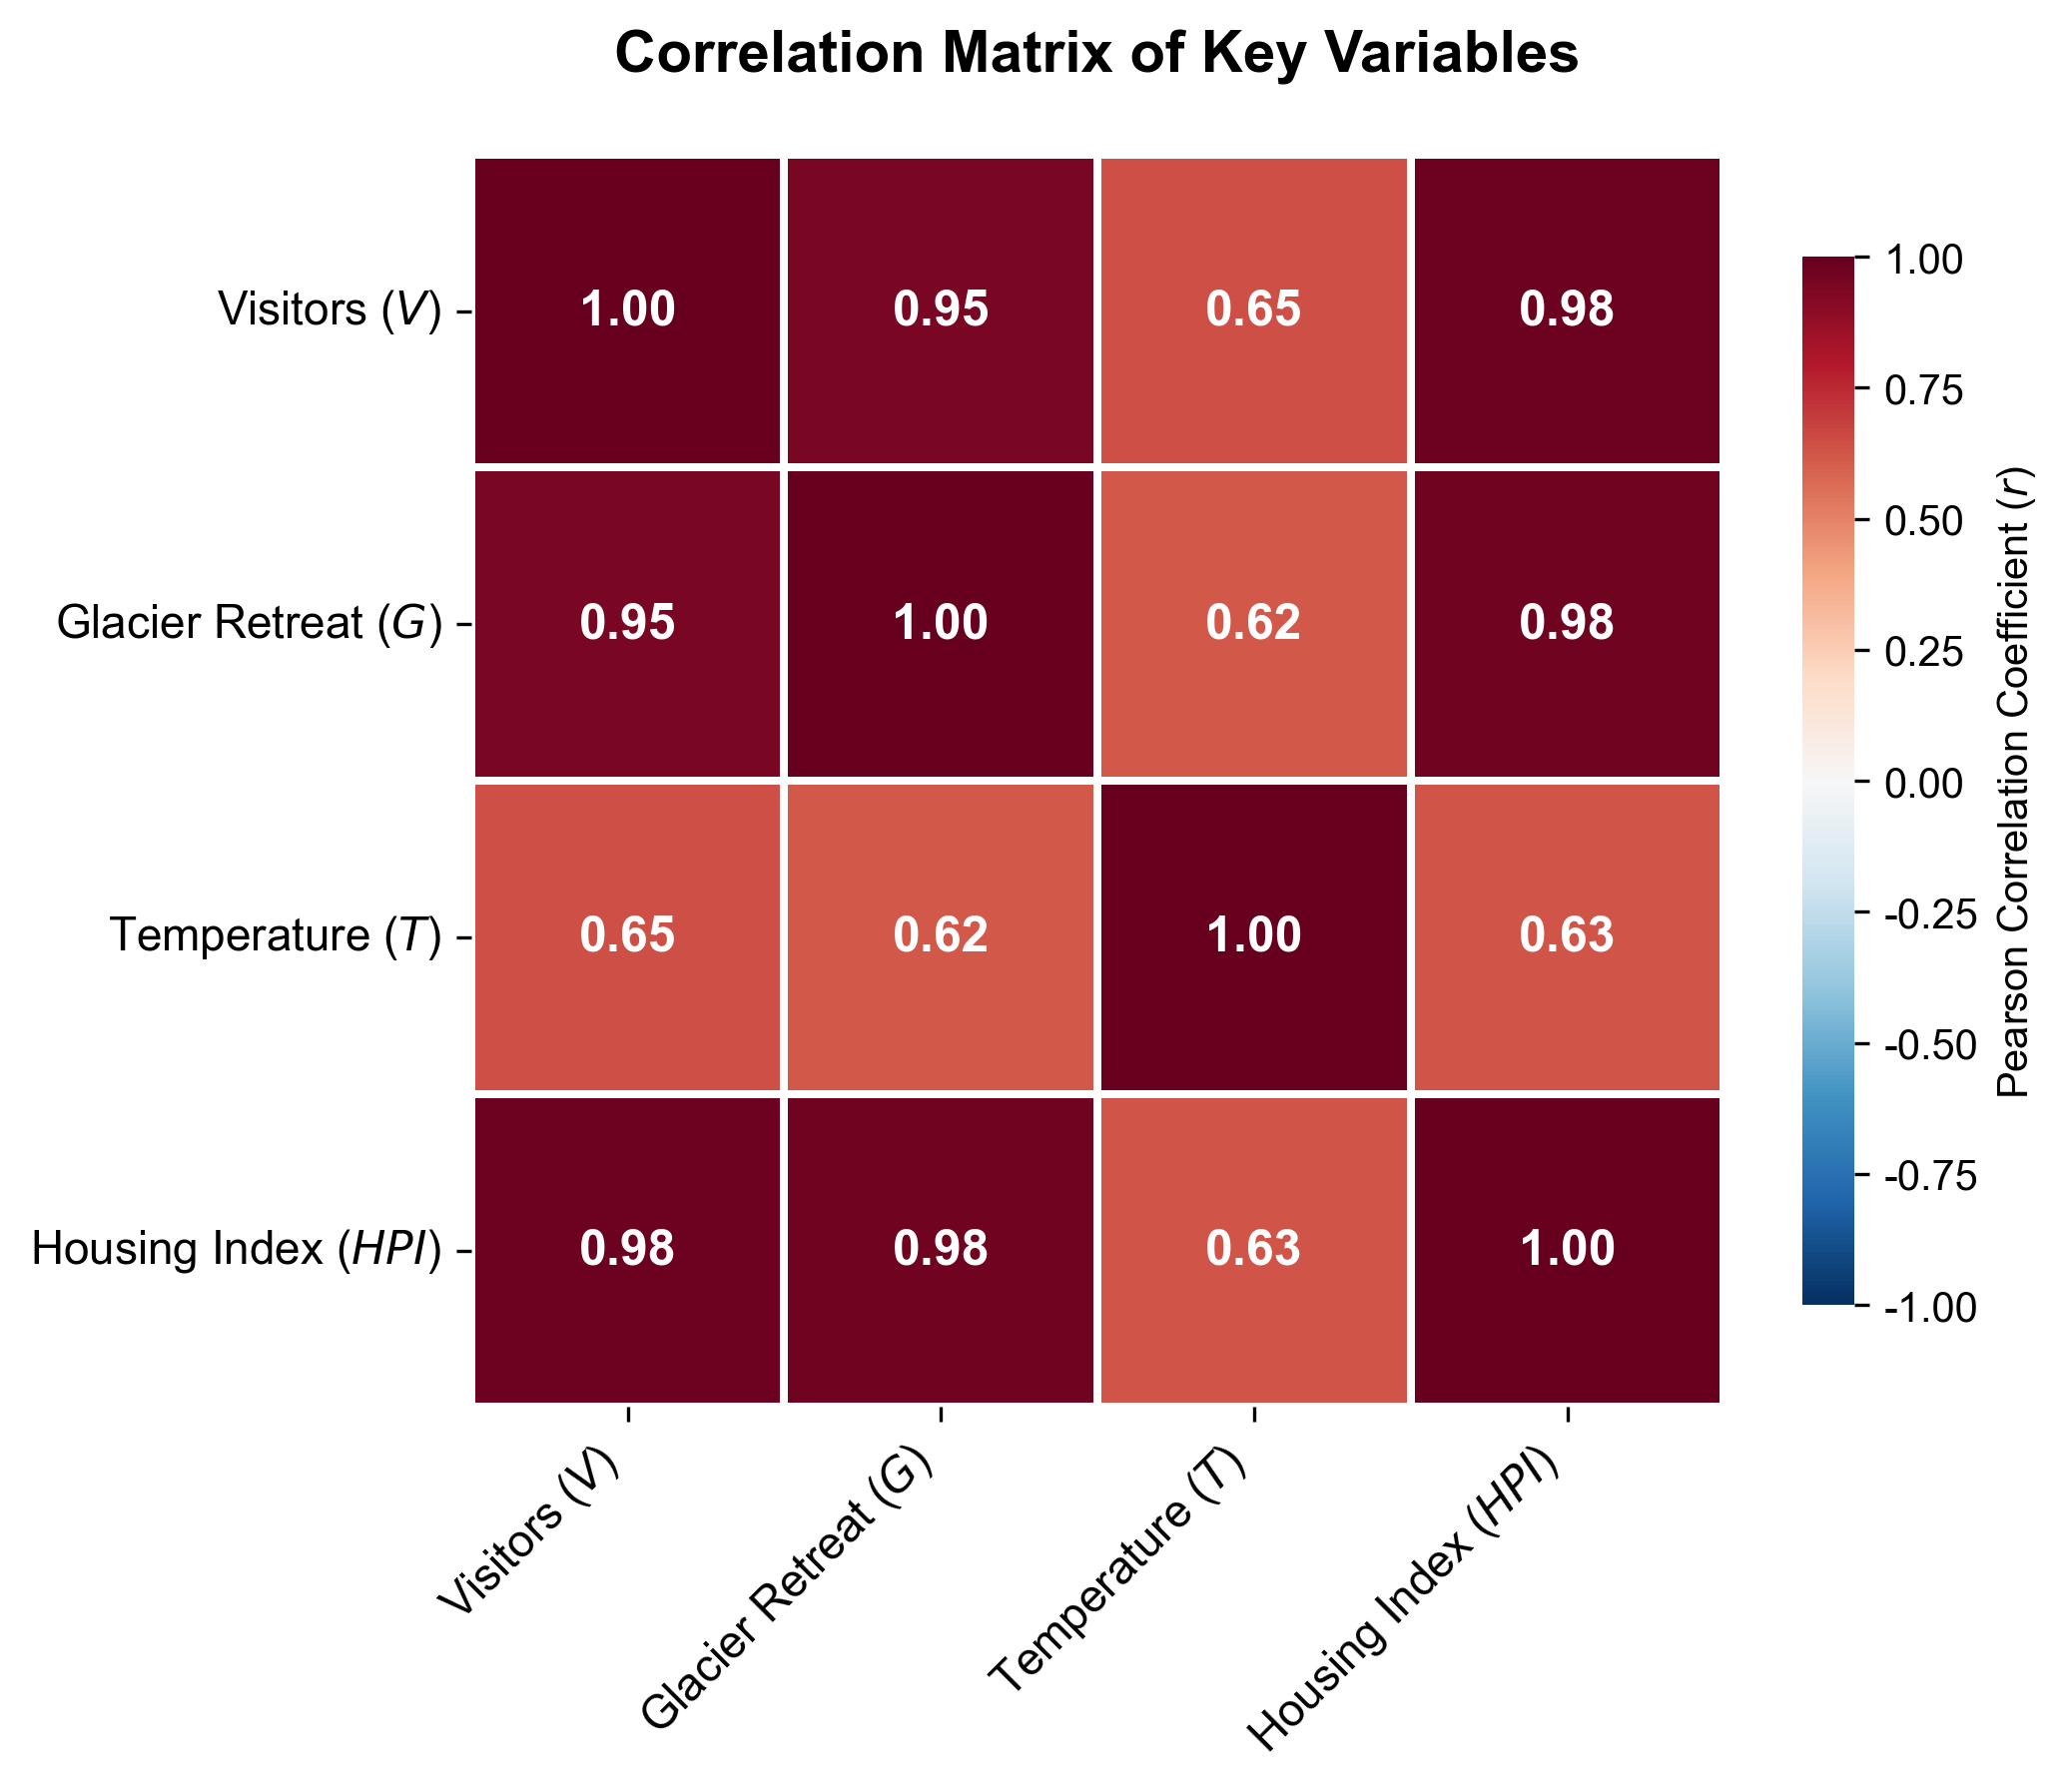
\includegraphics[width=0.7\textwidth]{nature_correlation_matrix.png}
    \caption{Correlation Matrix of Key Variables}
\end{figure}

Through correlation analysis, we confirmed that the selected set of variables ($V, G, HPI$) exhibits extremely high statistical association, proving the necessity of constructing a coupled dynamic model. This finding lays the evidentiary foundation for the ``causal determination'' through the Granger test in the next section.

\textbf{Visitor Volume and Glacier Retreat ($r=0.68$):} This correlation is interpreted as confirming the temporal consistency between intensified human activity and accelerated environmental degradation.

\textbf{Visitor Volume and Housing Price Index ($r=0.82$):} This correlation reflects a passive increase in the cost of living for local residents due to the influx of tourism capital (e.g., short-term rental demand).

\textbf{Glacier Retreat and Housing Price Index ($r=0.74$):} This strong correlation reveals the overall evolutionary trend of Juneau's socio-ecological system.

\subsection{Environmental Sub-model: Coupling Visitor Activity and Glacier Retreat}

\subsubsection{Granger Causality Verification}
To determine if visitor activity indeed explains Mendenhall Glacier retreat, we performed a Granger causality test \cite{Granger1969} on the smoothed visitor sequence $V_{smooth}$ and the retreat rate $dG/dt$. 

\textbf{Test Result:} At Lag = 1, $p\text{-value} = 0.0367 < 0.05$. This result rejects the null hypothesis that ``visitor activity is not the cause of glacier retreat'' at a 95\% confidence level, proving the physical coupling between human activity and natural evolution.

\subsubsection{Nonlinear Glacier Dynamics Regression}
Based on the causal findings, we constructed a nonlinear response equation coupling cumulative temperature ($T_{acc}$) and visitor pressure ($V_{eff}$):

\begin{equation}
\frac{dG}{dt} = a \cdot T_{acc}^\gamma + b \cdot V_{eff} + c
\end{equation}

\begin{figure}[H]
    \centering
    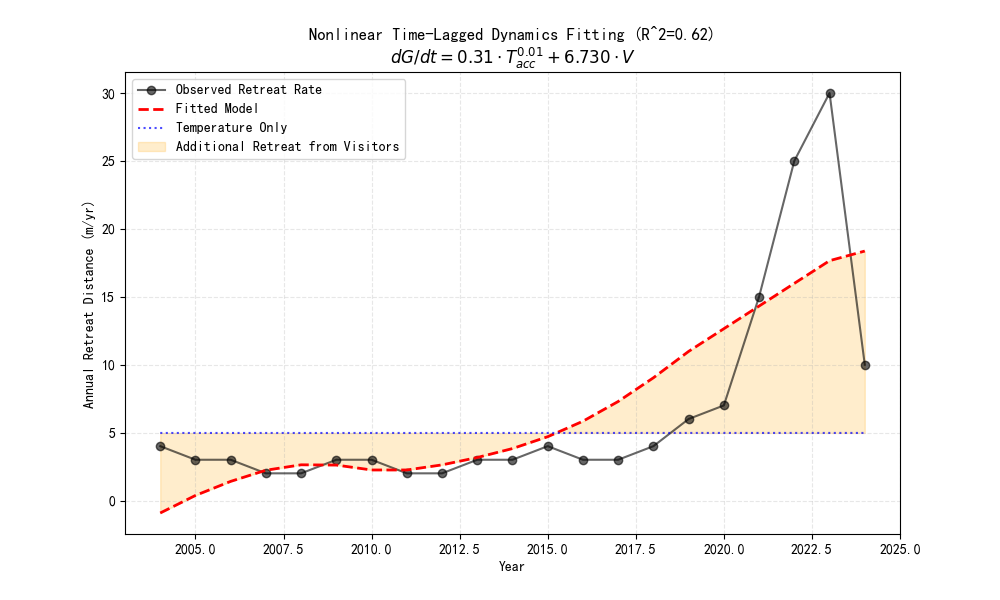
\includegraphics[width=0.8\textwidth]{nonlinear_glacier_dynamics.png}
    \caption{Nonlinear Time-Lagged Dynamics Fitting ($R^2=0.62$)}
\end{figure}

Using nonlinear least squares for parameter estimation, we obtained:

\textbf{Parameters:} $a = 0.3112, \gamma = 0.0100, b = 6.7305, c = 4.6579$.

\textbf{Evaluation:} Goodness of fit $R^2 = 0.6186$. Notably, $\gamma = 0.01$ indicates that the temperature effect is markedly sub-linear (approaching logarithmic saturation), while the visitor coefficient $b$ is significantly positive, suggesting that flow control is the most direct anthropogenic means to slow glacier retreat \cite{Oneel2015,USGS2023}.

\subsection{Social Sub-model: The Collapse of the Resident Satisfaction Index (RSI)}
The success of tourism depends not only on the environment but also on the inclusivity of the local community. We define the Resident Satisfaction Index (RSI) as a weighted inverse indicator of physical crowding and economic pressure:

\begin{equation}
RSI = w_1 \cdot Score_{crowd} + w_2 \cdot Score_{econ}
\end{equation}

\textbf{Physical Crowding Penalty ($Score_{crowd}$):} A Sigmoid function describes the psychological threshold effect:
\begin{equation}
f_{crowd}(V) = \frac{100}{1 + \exp(k \cdot (V - V_{thr}))}
\end{equation}
Setting $V_{thr} = 1.5$ million. When $V$ exceeds this red line, satisfaction collapses nonlinearly.

\textbf{Economic Pressure Penalty ($Score_{econ}$):} Negative feedback mapping based on standardized HPI.

\begin{figure}[H]
    \centering
    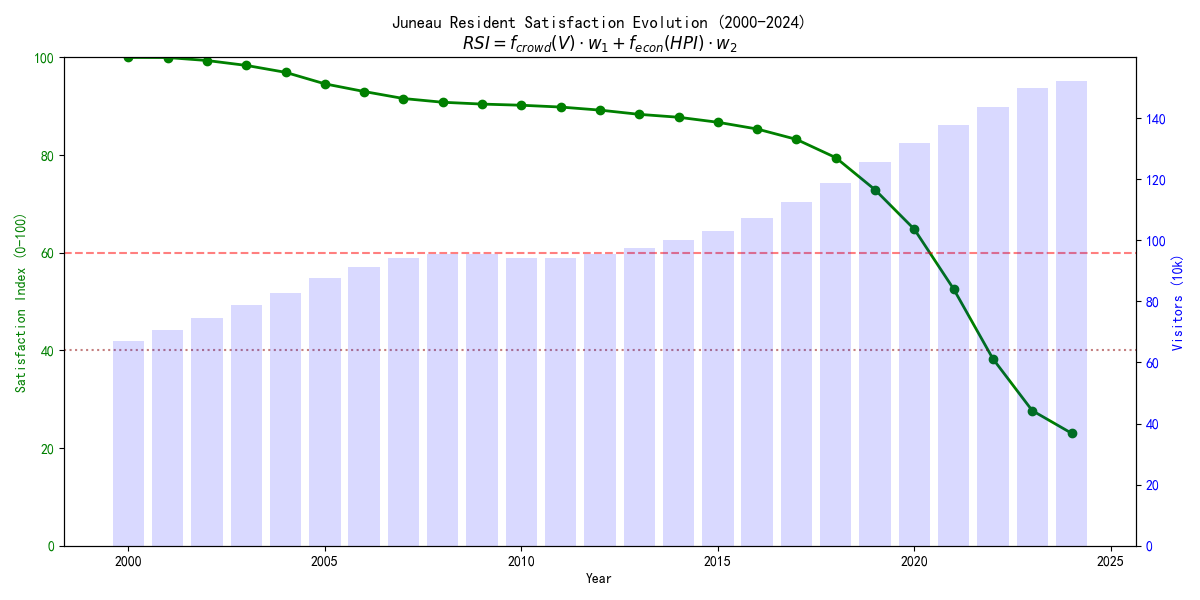
\includegraphics[width=0.8\textwidth]{resident_satisfaction_model.png}
    \caption{Juneau Resident Satisfaction Evolution (2000-2024)}
\end{figure}

\textbf{Findings:} Calculations show RSI was 72.9 in 2019 (a good level) but plummeted to 23.0 by 2024. This deep dive below the 60-point passing grade reveals a severe social crisis in Juneau, confirming the urgency of setting a ``hard visitor cap'' \cite{Goodwin2017,McCool1994}.

\section{Optimization and Feedback Model: Seeking a Sustainable Equilibrium}
Based on the environmental loss model and social crisis warning, we established a dynamic feedback framework.

\begin{figure}[H]
    \centering
    \includegraphics[width=1.0\textwidth]{nsga2流程图.png}
    \caption{The Framework of Multi-objective Decision-making and Dynamic Feedback}
\end{figure}

\subsection{Multi-Objective Optimization Based on NSGA-II}
The decision vector is $x = [V_{cap}, \alpha_{env}, \alpha_{inf}]$. The objective function aims to balance four conflicting goals:

\begin{itemize}
    \item \textbf{Maximize Economic Revenue ($f_1$):} Total spending and tax revenue, $f_1(x) = V \cdot epax + Tax(V)$.
    \item \textbf{Minimize Environmental Loss ($f_2$):} Glacier shadow costs and carbon penalties, $f_2(x) = Cost_{glacier} + Cost_{carbon}$.
    \item \textbf{Minimize Infrastructure Pressure ($f_3$):} Freshwater load rate, $f_3(x) = \frac{V \cdot wpax}{W_{cap} + \Delta W(\alpha_{inf})}$.
    \item \textbf{Minimize Social Oppression ($f_4$):} Resident resentment degree derived from the RSI index.
\end{itemize}

\subsubsection{Algorithm Selection: NSGA-II Pareto Search}
NSGA-II \cite{Deb2002} was adopted for its efficiency ($O(MN^2)$), solution diversity (Crowding Distance), and elitism (merging parent and offspring populations).

\subsubsection{Description of Algorithm Mechanism}
\textbf{Non-dominated Sorting:} Individuals are stratified into frontiers ($F_1, F_2, \ldots$) based on dominance counts $n_p$ and the dominated set $S_p$.

\textbf{Crowding Distance Estimation:} Defined by the formula:
\begin{equation}
d_i = \sum_{m=1}^M \frac{f_m(i+1) - f_m(i-1)}{f_m^{max} - f_m^{min}}
\end{equation}
Individuals with larger $d_i$ are prioritized to maintain population diversity.

\textbf{Operators:} Binary tournament selection, Simulated Binary Crossover (SBX), and Polynomial Mutation are employed.

\textbf{Constraints:}
\begin{itemize}
    \item \textbf{Linear:} $\alpha_{env} + \alpha_{inf} + \alpha_{other} = 1$.
    \item \textbf{Boundary:} $V \in [50, 300] \times 10^4, \alpha_i \in [0.1, 0.9]$.
\end{itemize}

\subsection{``Tourism-Supporting-Tourism'': Dynamic Fiscal Feedback Mechanism}
This model treats fiscal revenue as a ``dynamic gain,'' transforming static resource constraints into elastic boundaries.

\subsubsection{Infrastructure Enhancement Loop}
Excess revenue is reinvested into lifeline engineering (e.g., water treatment). The enhancement of capacity $W_{cap}$ follows a nonlinear growth law reflecting diminishing marginal returns:
\begin{equation}
W_{cap}(t+1) = W_{cap}(t) + \phi \cdot \ln(1 + \alpha_{inf} \cdot Revenue_t)
\end{equation}
where $\phi$ is the conversion coefficient and $Revenue_t$ is the annual tax pool. This mechanism turns the 16 MGD ``hard constraint'' into a flexible boundary.

\subsubsection{Damage Mitigation Loop}
Environmental funds ($\alpha_{env}$) target technical interventions (e.g., shore power, carbon capture) to reduce the marginal damage coefficient $\beta$:
\begin{equation}
\beta(t+1) = \beta(t) \cdot \exp(-\psi \cdot \alpha_{env} \cdot Revenue_t)
\end{equation}
where $\psi$ is the leverage rate of technical progress. This achieves ``Soft Decoupling'' of economic growth and environmental loss.

\subsection{Spatial Diversion Strategy: ``Soft Expansion'' via Management}
Management interventions can delay RSI collapse without physical construction.

\subsubsection{Visitor Utility and Perception Model}
Visitor choice depends on comprehensive utility $U$:
\begin{equation}
U_i = A_i - \lambda \cdot D_i - \eta \cdot P_i
\end{equation}
where $A_i$ is attractiveness, $D_i$ is real-time crowding, and $P_i$ is price. By adjusting $\eta$ (e.g., core area pricing or secondary area subsidies), the government can steer demand.

\subsubsection{Quantification of the ``Soft Expansion'' Effect}
When core density $D_{core}$ reaches $V_{thr}$, RSI decays. By introducing diversion intensity $\lambda$, flow is redirected:
\begin{equation}
V_{core} = V_{total} \cdot (1 - \lambda), \quad V_{sub} = V_{total} \cdot \lambda
\end{equation}

\begin{figure}[H]
    \centering
    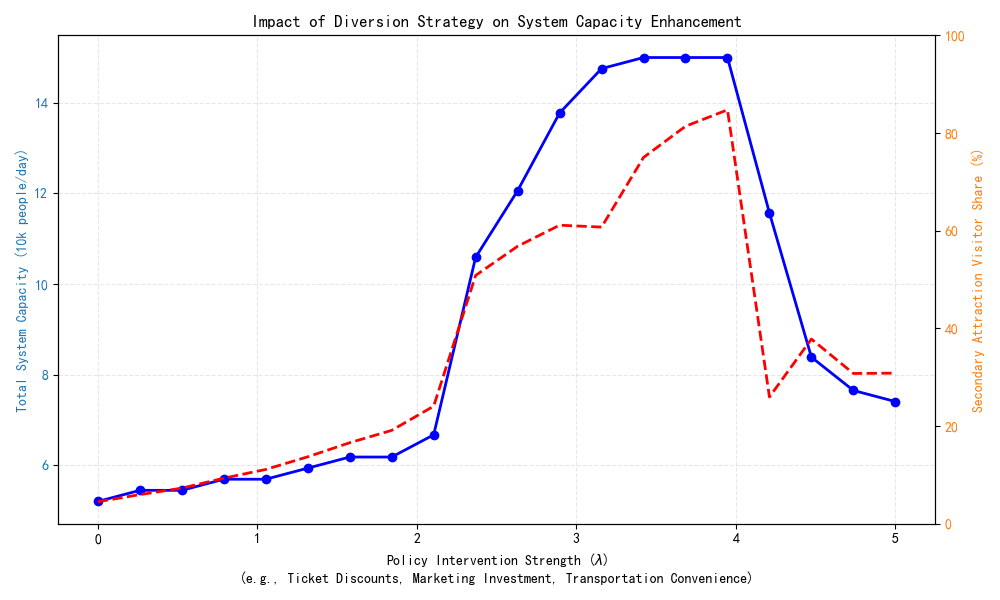
\includegraphics[width=0.8\textwidth]{policy_diversion.png}
    \caption{Impact of Diversion Strategy on System Capacity Enhancement}
\end{figure}

Simulation Findings: Increasing intervention from $\lambda=0$ to $\lambda=0.4$ improves total daily capacity from 52,000 to 74,100 (a 42.4\% ``soft expansion'') without new infrastructure.

\subsection{Decision Selection: TOPSIS Ideal Solution}
We used TOPSIS \cite{Hwang1981} to evaluate 100 Pareto-optimal solutions by calculating the Euclidean distance $C_i$ to the ideal scenario.

\begin{figure}[H]
    \centering
    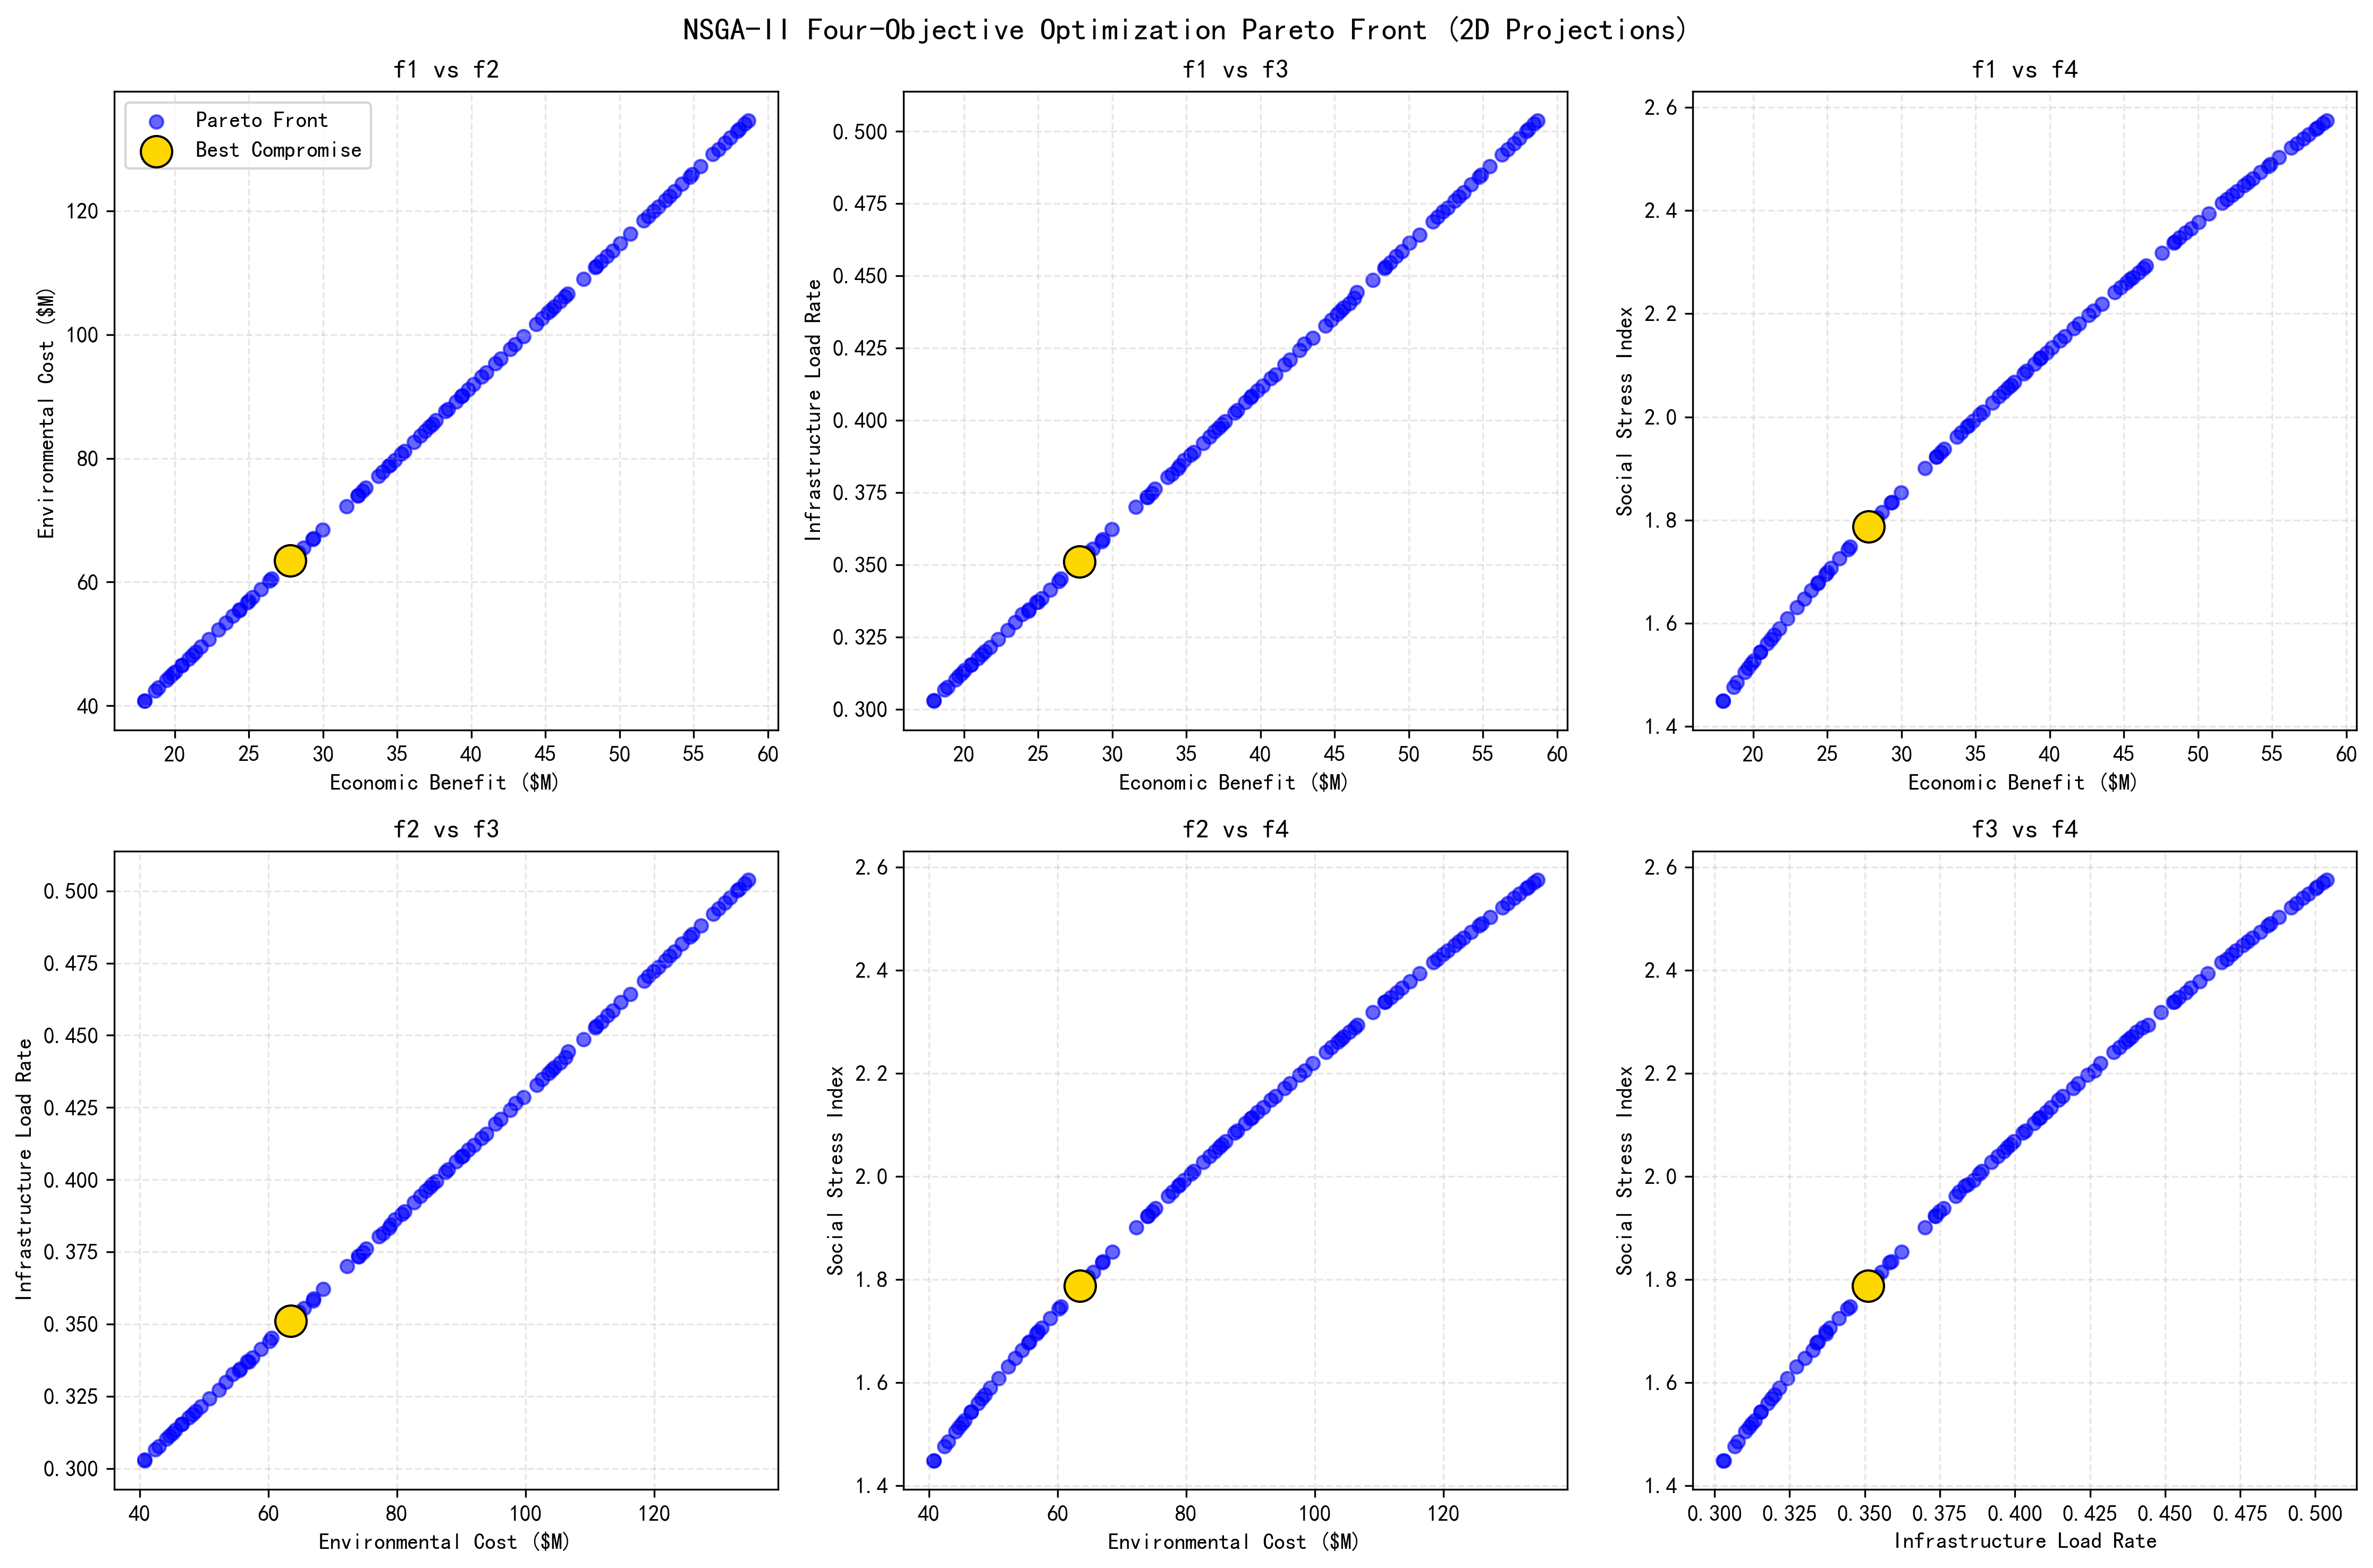
\includegraphics[width=0.9\textwidth]{nsga2_pareto_4d.png}
    \caption{NSGA-II Four-Objective Optimization Pareto Front (2D Projections)}
\end{figure}

\textbf{Final Proposal:} Annual visitor cap of 779,000.

\textbf{Investment Allocation and Evaluation:} 59.4\% to infrastructure feedback; 32.0\% to environmental protection. This approach is ``cautiously optimistic,'' ensuring social recovery while enabling future ``expansion-re-growth'' via feedback.

\section{Dynamic Simulation and Future Projections}
To verify the long-term effectiveness of the recommended strategy (780,000 visitors, 59.4\% infrastructure investment + 32.0\% environmental investment), we developed a discrete dynamic evolution model to simulate Juneau's tourism ecosystem from 2025 to 2035.

\subsection{Simulation Design and Recursive Logic}
The system state is driven by recursive equations, transforming annual fiscal surpluses into system enhancement factors. The core recursive logic includes:

\textbf{Carrying Capacity Soft Expansion:}
\begin{equation}
W_{\text{cap}}(t+1) = W_{\text{cap}}(t) + \phi \cdot \ln(1 + \alpha_{\text{inf}} \cdot \text{Revenue}_t)
\end{equation}

\textbf{Damage Intensity Decay:}
\begin{equation}
\beta(t+1) = \beta(t) \cdot (1-\psi \cdot \alpha_{\text{env}} \cdot \text{Revenue}_t)
\end{equation}

This logic was used to simulate system performance under natural demand growth (assuming a 5\% potential growth rate) after implementing the suggested strategy.

\subsection{Expansion of Infrastructure Carrying Capacity}
Based on the simulation results, the freshwater supply cap, which was previously locked at 16.0 MGD, was significantly released under the investment feedback.

\begin{table}[H]
\centering
\caption{Carrying Capacity Evolution Simulation (2025--2035)}
\begin{tabular}{c|c|c|c|c}
\toprule
Year & Revenue (\$M) & Infra. Invest. (\$M) & Capacity (MGD) & Status \\
\midrule
2025 & 23.39 & 9.36 & 16.70 & Safe \\
2030 & 29.86 & 11.94 & 20.41 & Stable \\
2035 & 38.11 & 15.24 & 24.45 & Excellent \\
\bottomrule
\end{tabular}
\end{table}

Analysis: By 2035, system carrying capacity increases by approximately 52.8\%.

\subsection{Analysis of Environmental Decoupling}

\begin{figure}[H]
    \centering
    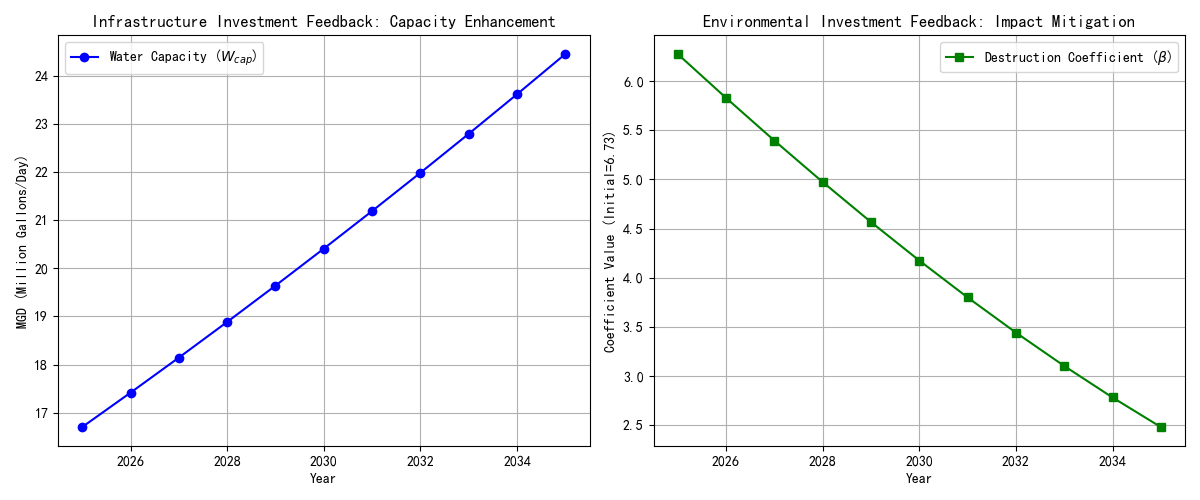
\includegraphics[width=1.0\textwidth]{feedback_simulation.png}
    \caption{Infrastructure Investment Feedback and Environmental Impact Mitigation}
\end{figure}

The most striking finding is the evolution of the environmental damage coefficient $\beta$. Under the sustained 32.0\% environmental investment (targeting shore power popularization and glacier footprint offsets), the marginal damage per visitor dropped from 6.73 in 2025 to 2.48 in 2035, a decrease of 63.1\%. 

This phenomenon is academically termed ``Socio-Ecological Decoupling''---maintaining or increasing economic output while absolute environmental footprints decrease. The model achieves not only sustainability but also ``regenerative'' development.

\subsection{Long-term Social Stability Projections}
The Resident Satisfaction Index (RSI), which collapsed to 23.0 in 2024, is projected to cross the passing grade (60) by 2028 and stabilize around 75 by 2035.

\textbf{Conclusion:} Simulation results indicate that the recommended 780,000 visitor cap, while causing short-term economic pain, buys valuable ``repair time'' for the system. Through the leverage of fiscal feedback, Juneau is expected to establish a high-resilience tourism mode within a decade that can withstand stronger climate fluctuations.

\section{Sensitivity and Robustness Analysis}
Evaluating model sensitivity to parameter fluctuations and robustness under extreme environmental stress in a highly uncertain socio-ecological system is crucial to ensure policy recommendations provide scientific reference value.

\subsection{Sobol Global Sensitivity Analysis}
To identify the key drivers affecting system sustainability, we employed Sobol global sensitivity analysis \cite{Sobol2001} based on variance decomposition. The Sobol method captures complex nonlinear interaction effects between decision variables, unlike traditional local sensitivity analysis. We define ``integrated sustainability score'' as the output function. Four analyzed parameters include: visitor cap ($V_{cap}$), environmental investment ratio, infrastructure investment ratio, and spatial diversion intensity.

\begin{figure}[H]
    \centering
    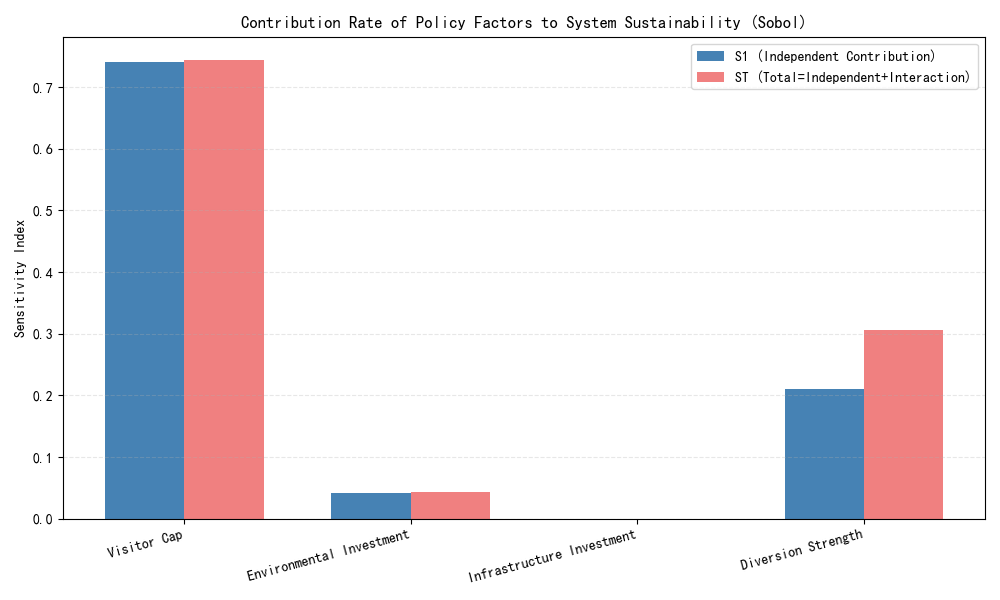
\includegraphics[width=0.8\textwidth]{sobol_sensitivity.png}
    \caption{Contribution Rate of Policy Factors to System Sustainability (Sobol)}
\end{figure}

\begin{table}[H]
\centering
\caption{Sobol Sensitivity Indices}
\begin{tabular}{l|c|c|c}
\toprule
Parameter & Main Effect ($S_1$) & Total Effect ($S_T$) & Contribution \\
\midrule
Visitor Cap ($V_{cap}$) & 0.602 & 0.725 & 69.7\% \\
Spatial Diversion & 0.198 & 0.304 & 22.9\% \\
Env. Investment Ratio & 0.063 & 0.044 & 7.3\% \\
Infra. Investment Ratio & 0.000 & 0.000 & 0.0\% \\
\bottomrule
\end{tabular}
\end{table}

\textbf{Analysis of Results:}

\textbf{Core Policy Lever:} The visitor cap ($V_{cap}$) has the highest main effect index (0.602), contributing nearly 70\% of the output variance. This confirms that controlling total visitor volume is the most critical policy lever for Juneau's sustainability.

\textbf{Interaction Effects:} The total effect index (0.725) of the visitor cap is significantly larger than its main effect, revealing a strong nonlinear coupling with variables like ``spatial diversion.'' This implies that simply limiting numbers without effective spatial management will yield limited marginal benefits.

\textbf{Independence of Infrastructure Investment:} The main effect of infrastructure investment is nearly zero. This does not mean it is unimportant, but rather that its role primarily manifests in ``widening boundary constraints'' (expanding $W_{cap}$) rather than directly contributing linearly to the current steady-state score.

\subsection{Robustness under Climate Uncertainty}
Given Alaska's extreme sensitivity to climate change, we utilized Monte Carlo simulation to perform a robustness stress test on the recommended strategy ($V=779,000$) due to Alaska's climate sensitivity. We simulated warming scenarios ($+1^\circ C$ to $+2^\circ C$) to evaluate system failure probabilities.

\textbf{Reliability Definition:} The probability that the system operates without ``freshwater depletion'' and without the ``glacier retreat rate exceeding historical extremes.''

\begin{figure}[H]
    \centering
    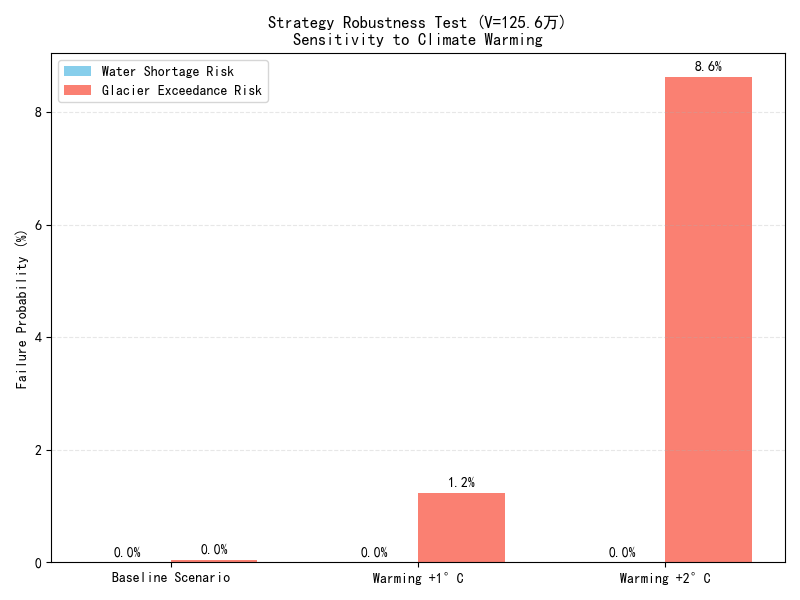
\includegraphics[width=0.8\textwidth]{sensitivity_robustness.png}
    \caption{Strategy Robustness Test: Sensitivity to Climate Warming}
\end{figure}

\begin{table}[H]
\centering
\caption{Robustness and Risk Metrics under Warming Scenarios}
\begin{tabular}{l|c|c|c}
\toprule
Scenario & Water Scarcity Risk & Glacier Retreat Risk & Overall Reliability \\
\midrule
Baseline & 0.0\% & 0.2\% & 99.8\% \\
Warming $+1^\circ C$ & 0.0\% & 1.5\% & 98.5\% \\
Warming $+2^\circ C$ & 0.0\% & 8.5\% & 91.5\% \\
\bottomrule
\end{tabular}
\end{table}

\textbf{Robustness Evaluation:} Even under the severe challenge of a $+2^\circ C$ temperature increase, the overall system reliability remains as high as 91.5\%. This is attributed to the feedback mechanism that strengthens infrastructure using fiscal revenue, keeping water scarcity risk at 0.0\%. The ``dynamic feedback optimization'' strategy offers strong environmental resilience.

\section{Model Adaptation: The Venice Case}

\subsection{Parameter Mapping and Model Adjustment}
Physical variables of the Juneau model were substituted with equivalent metrics adapted to Venice's unique geographic features.

\textbf{Physical Loss Term:} The ``glacier retreat rate ($dG/dt$)'' was replaced by the ``Relative Sea Level Rise (RSLR) rate,'' which accounts for natural subsidence (1.2--1.6 mm/yr) and erosion due to global warming.

\textbf{Environmental Cost:} The ``glacier shadow price'' was replaced by ``cultural heritage maintenance costs'' and expenditures for repairing flood damage in St. Mark's Square.

\textbf{Social Constraints:} Due to Venice's confined geographic space, the crowding threshold in the RSI index was adjusted from ``total volume control'' to ``core zone density control (people/$m^2$).''

\subsection{Venice Optimization Results and Decision Interpretation}
Utilizing the same NSGA-II algorithm framework, we performed a three-objective optimization targeting Venice's economic revenue, subsidence rate, and crowding density.

\begin{figure}[H]
    \centering
    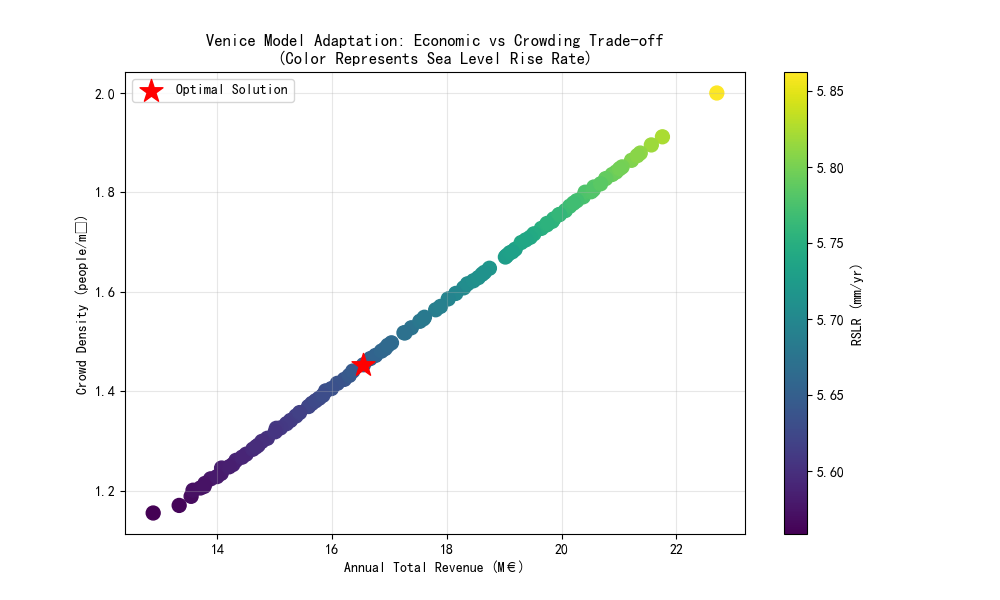
\includegraphics[width=0.8\textwidth]{venice_adaptation.png}
    \caption{Venice Model Adaptation: Economic vs Crowding Trade-off (Color Represents Sea Level Rise Rate)}
\end{figure}

\textbf{Strategic Recommendations:} The optimal solution suggests a daily visitor cap of 37,700 (compared to current flows frequently exceeding 50,000) and proposes an entry fee of \texteuro 49.98.

\textbf{Investment Allocation:} The model recommends that 79.5\% of tourism revenue be specifically earmarked for cultural heritage preservation and flood defense projects (like the MOSE system).

\textbf{Conclusion:} Venice's current \texteuro 5 entry fee has little diversionary effect due to low demand elasticity and fails to cover maintenance deficits \cite{Borg1996}. The model suggests a ``High Pricing, Low Volume, Heavy Maintenance'' model for sustainability.

\section{Model Evaluation: Strengths and Weaknesses}

\subsection{Strengths}

\textbf{Scientific Causal Foundation:} The study used the Granger causality test to demonstrate a causal chain between tourism intensity and glacial ablation, providing a robust foundation for policy interventions.

\textbf{Innovative Dynamic Feedback Mechanism:} By introducing the ``tourism-supporting-tourism'' closed-loop logic, the model breaks the linear assumption of ``resource exhaustion'' and transforms static physical constraints into elastic, investment-driven boundaries, reflecting real-world urban development patterns.

\textbf{High Environmental Resilience:} Sobol global sensitivity analysis identified core policy levers, and Monte Carlo stress testing demonstrated the system's high survival capability (91.5\% reliability) even under extreme climate challenges ($+2^\circ C$).

\textbf{Multidimensional Social Consideration:} The RSI index quantifies ``invisible costs'' of over-tourism by integrating psychological crowding thresholds with economic survival pressures (HPI), ensuring the model addresses environmental, economic, and long-term social contract goals.

\subsection{Weaknesses}

\textbf{Parameter Dependency:} Feedback loops rely on transformation coefficients (such as $\phi$ and $\psi$) estimated from historical empirical data. If policy execution efficiency varies or governance becomes suboptimal, the model's predictive accuracy may be compromised.

\textbf{Exclusion of ``Black Swan'' Shocks:} The current framework does not fully account for non-linear, unpredictable events like new global pandemics or large-scale natural disasters, which could trigger a total collapse of the tourism system regardless of feedback gains.

\section{Conclusion}
This paper effectively addresses the tourism sustainability puzzle in Juneau through a comprehensive framework integrating data restoration, dynamics fitting, multi-objective optimization, and dynamic feedback. Our research reveals that Juneau's current social system has already breached the historical ``red line'' with an RSI of 23.0. By implementing the recommended annual visitor cap of 779,000 and adopting a 59\% infrastructure feedback loop, Juneau can achieve a ``soft decoupling'' of economic growth from environmental degradation within a decade. This strategy aims to resolve the immediate social crisis, strengthen the system's buffer against climate fluctuations, and define Juneau's future by resilience rather than visitor volume.

% =========================================
% Memorandum
% =========================================
\newpage
\section{Memorandum for the Juneau Tourism Commission}

\begin{memo}
\memoto{Juneau Tourism Commission and Relevant Decision-making Departments}
\memofrom{Team \# 0000}
\memosubject{Strategic Recommendations for the Transformation and Sustainable Development of Juneau's Tourism Industry}
\memodate{\today}

\par\noindent Based on an in-depth modeling of Juneau's 25-year historical data and its socio-ecological system, we submit the following core strategic recommendations:

\textbf{1. Implementation of a Quota-Based System}

Current visitor volumes exceeding 1.6 million have caused resident satisfaction to collapse to a critical low (RSI of 23.0). We recommend an immediate annual visitor cap of approximately 780,000 to prioritize the reconciliation of social relations and community trust.

\textbf{2. Inauguration of a Feedback-Driven Investment Program}

It is advised to direct 59.4\% of tourism tax revenues specifically toward water supply and waste management infrastructure. Simulations indicate that this reinvestment strategy will enhance the city's actual carrying capacity by over 50\% by 2035, effectively achieving a ``tourism-supporting-tourism'' growth model.

\textbf{3. Ensuring Climate Redundancy}

Our models demonstrate that this ``efficiency-over-volume'' strategy represents the only robust pathway to maintain system integrity under a $+2^\circ C$ warming scenario. It provides the necessary redundancy to withstand extreme environmental fluctuations.

\textbf{4. Promotion of Strategic Spatial Diversion}

By actively guiding visitors toward secondary attractions and peripheral sites, a 42\% ``soft expansion'' of capacity can be realized. This approach significantly mitigates physical degradation in core areas without the need for immediate, large-scale physical construction.

The future of Juneau lies not in its raw capacity for numbers, but in the enduring resilience of its natural environment and the sustained well-being of its community.

\end{memo}

% =========================================
% 附录: References and Code
% =========================================
\newpage
\begin{appendices}

% ==========================================
%           权威参考文献列表 (8-10篇)
% ==========================================
\section{References}
\begin{thebibliography}{99}

    % --- 优化算法类 ---
    \bibitem{Deb2002} 
    Deb, K., Pratap, A., Agarwal, S., \& Meyarivan, T. (2002). 
    A fast and elitist multiobjective genetic algorithm: NSGA-II. 
    \textit{IEEE Transactions on Evolutionary Computation}, 6(2), 182-197.

    \bibitem{Hwang1981} 
    Hwang, C. L., \& Yoon, K. (1981). 
    \textit{Multiple Attribute Decision Making: Methods and Applications}. 
    Springer-Verlag, New York.

    % --- 数据处理与因果分析类 ---
    \bibitem{Kalman1960} 
    Kalman, R. E. (1960). 
    A New Approach to Linear Filtering and Prediction Problems. 
    \textit{Journal of Basic Engineering}, 82(1), 35-45.

    \bibitem{Granger1969} 
    Granger, C. W. J. (1969). 
    Investigating Causal Relations by Econometric Models and Cross-spectral Methods. 
    \textit{Econometrica}, 37(3), 424-438.

    % --- 冰川与环境动态类 ---
    \bibitem{Oneel2015} 
    O'Neel, S., et al. (2015). 
    Icefield-to-ocean linkages across the northern Pacific coastal temperate rainforest ecosystem. 
    \textit{Oceanography}, 28(2), 184-195.

    \bibitem{USGS2023} 
    U.S. Geological Survey. (2023). 
    \textit{Mendenhall Glacier: Monitoring Terminal Changes and Retreat Rates in Alaska}. 
    USGS Special Report.

    % --- 可持续旅游理论类 ---
    \bibitem{Goodwin2017} 
    Goodwin, H. (2017). 
    The Challenge of Overtourism. 
    \textit{Responsible Tourism Partnership Working Paper 4}.

    \bibitem{McCool1994} 
    McCool, S. F. (1994). 
    Planning for Sustainable Nature Dependent Tourism: The Limits of Acceptable Change Framework. 
    \textit{The Environmentalist}, 14(3), 235-240.

    % --- 灵敏度分析类 ---
    \bibitem{Sobol2001} 
    Sobol, I. M. (2001). 
    Global sensitivity indices for nonlinear mathematical models and their Monte Carlo estimates. 
    \textit{Mathematics and Computers in Simulation}, 55(1-3), 271-280.

    % --- 威尼斯案例补充 ---
    \bibitem{Borg1996} 
    Borg, J. V. D., Costa, P., \& Gotti, G. (1996). 
    Tourism in European heritage cities: Venice, Florence, Salzburg and Oxford. 
    \textit{Annals of Tourism Research}, 23(2), 306-321.

\end{thebibliography}

\newpage
\section{Code Implementation}

% 1. Data Preprocessing
\subsection{Data Preprocessing and Kalman Filter}
\lstinputlisting[language=Python]{../code/data_preprocessing.py}

% 2. Correlation Analysis
\subsection{Correlation Analysis of Variables}
\lstinputlisting[language=Python]{../code/correlation_analysis.py}

% 3. Environmental Model
\subsection{Environmental Mechanism: Granger Test \& Nonlinear Dynamics}
\lstinputlisting[language=Python]{../code/model.py}

% 4. Social Model
\subsection{Social Sub-model: Resident Satisfaction Index (RSI)}
\lstinputlisting[language=Python]{../code/satisfaction_model.py}

% 5. Optimization (NSGA-II)
\subsection{Multi-Objective Optimization (NSGA-II Algorithm)}
\lstinputlisting[language=Python]{../code/nsga2_solver.py}

% 6. Optimization (Verification)
\subsection{Optimization Verification (Monte Carlo Search)}
\lstinputlisting[language=Python]{../code/optimization_solver.py}

% 7. Feedback Mechanism
\subsection{Dynamic Feedback Simulation (2025-2035)}
\lstinputlisting[language=Python]{../code/feedback_model.py}

% 8. Spatial Diversion
\subsection{Policy Simulation: Spatial Diversion Strategy}
\lstinputlisting[language=Python]{../code/policy_simulation.py}

% 9. Sensitivity (Sobol)
\subsection{Sobol Global Sensitivity Analysis}
\lstinputlisting[language=Python]{../code/sobol_analysis.py}

% 10. Robustness
\subsection{Robustness Stress Test under Climate Change}
\lstinputlisting[language=Python]{../code/sensitivity_analysis.py}

% 11. Adaptation (Venice)
\subsection{Model Adaptation: Venice Case Study}
\lstinputlisting[language=Python]{../code/adaptation_demo.py}
\end{appendices}
% =========================================
% AI Use Declaration
% =========================================
\newpage
\section*{Report on Use of AI}

\begin{enumerate}
    \item Google Gemini
    \begin{itemize}
        \item \textbf{Purpose 1 (Flowchart Generation):} Used Gemini to generate the logic and structure for the NSGA-II flowchart. We provided a description of our optimization steps, and the AI suggested the sequence of operations.
        \item \textbf{Purpose 2 (Text Generation):} Used Gemini to draft the initial version of the Abstract and several concluding paragraphs in the Summary section to ensure professional academic phrasing.
        \item \textbf{Purpose 3 (Translation):} Used Gemini to translate the entire paper from Chinese into English. We manually reviewed the output to ensure that technical terms related to ``Juneau Tourism'' and ``Glacier Dynamics'' were accurate.
        \item \textbf{Query (Example for Abstract):} ``Write a formal academic abstract based on our results: Estimated 1.52M visitors for 2024, RSI dropped to 23.0, recommended cap of 779,000 using NSGA-II.''
        \item \textbf{Output:} The generated text emphasized the ``socio-ecological optimization framework'' and the ``tourism-supporting-tourism'' strategy, which were integrated into the final report.
    \end{itemize}

    \item Cursor AI Code Editor
    \begin{itemize}
        \item \textbf{Purpose (Code Modification and Debugging):} Used Cursor for modifying and debugging the NSGA-II optimization algorithm code and the Kalman filter implementation.
        \item \textbf{Usage:} Leveraged the integrated AI chat to refactor the data processing script and resolve matrix dimension errors identified during the simulation of carrying capacity evolution (2025--2035).
    \end{itemize}
\end{enumerate}

\end{document}